\documentclass[10pt]{article}\usepackage[]{graphicx}\usepackage[]{color}
%% maxwidth is the original width if it is less than linewidth
%% otherwise use linewidth (to make sure the graphics do not exceed the margin)
\makeatletter
\def\maxwidth{ %
  \ifdim\Gin@nat@width>\linewidth
    \linewidth
  \else
    \Gin@nat@width
  \fi
}
\makeatother

\definecolor{fgcolor}{rgb}{0.345, 0.345, 0.345}
\newcommand{\hlnum}[1]{\textcolor[rgb]{0.686,0.059,0.569}{#1}}%
\newcommand{\hlstr}[1]{\textcolor[rgb]{0.192,0.494,0.8}{#1}}%
\newcommand{\hlcom}[1]{\textcolor[rgb]{0.678,0.584,0.686}{\textit{#1}}}%
\newcommand{\hlopt}[1]{\textcolor[rgb]{0,0,0}{#1}}%
\newcommand{\hlstd}[1]{\textcolor[rgb]{0.345,0.345,0.345}{#1}}%
\newcommand{\hlkwa}[1]{\textcolor[rgb]{0.161,0.373,0.58}{\textbf{#1}}}%
\newcommand{\hlkwb}[1]{\textcolor[rgb]{0.69,0.353,0.396}{#1}}%
\newcommand{\hlkwc}[1]{\textcolor[rgb]{0.333,0.667,0.333}{#1}}%
\newcommand{\hlkwd}[1]{\textcolor[rgb]{0.737,0.353,0.396}{\textbf{#1}}}%
\let\hlipl\hlkwb

\usepackage{framed}
\makeatletter
\newenvironment{kframe}{%
 \def\at@end@of@kframe{}%
 \ifinner\ifhmode%
  \def\at@end@of@kframe{\end{minipage}}%
  \begin{minipage}{\columnwidth}%
 \fi\fi%
 \def\FrameCommand##1{\hskip\@totalleftmargin \hskip-\fboxsep
 \colorbox{shadecolor}{##1}\hskip-\fboxsep
     % There is no \\@totalrightmargin, so:
     \hskip-\linewidth \hskip-\@totalleftmargin \hskip\columnwidth}%
 \MakeFramed {\advance\hsize-\width
   \@totalleftmargin\z@ \linewidth\hsize
   \@setminipage}}%
 {\par\unskip\endMakeFramed%
 \at@end@of@kframe}
\makeatother

\definecolor{shadecolor}{rgb}{.97, .97, .97}
\definecolor{messagecolor}{rgb}{0, 0, 0}
\definecolor{warningcolor}{rgb}{1, 0, 1}
\definecolor{errorcolor}{rgb}{1, 0, 0}
\newenvironment{knitrout}{}{} % an empty environment to be redefined in TeX

\usepackage{alltt}

\usepackage{amsmath,amssymb,amsthm}
\usepackage{fancyhdr,url}
\usepackage{graphicx}

\oddsidemargin 0in  %0.5in
\topmargin     0in
\leftmargin    0in
\rightmargin   0in
\textheight    9in
\textwidth     6in %6in
%\headheight    0in
%\headsep       0in
%\footskip      0.5in

\newtheorem{thm}{Theorem}
\newtheorem{cor}[thm]{Corollary}
\newtheorem{obs}{Observation}
\newtheorem{lemma}{Lemma}
\newtheorem{claim}{Claim}
\newtheorem{definition}{Definition}
\newtheorem{question}{Question}
\newtheorem{answer}{Answer}
\newtheorem{problem}{Problem}
\newtheorem{solution}{Solution}
\newtheorem{conjecture}{Conjecture}

\pagestyle{fancy}

\lhead{\textsc{MATH 141}}
\chead{\textsc{Practice}}
\rhead{\textsc{\today}}
\lfoot{}
\cfoot{}
%\cfoot{\thepage}
\rfoot{}
\renewcommand{\headrulewidth}{0.2pt}
\renewcommand{\footrulewidth}{0.0pt}

\newcommand{\ans}{\vspace{0.25in}}
\IfFileExists{upquote.sty}{\usepackage{upquote}}{}
\begin{document}

\paragraph{Millennials and Marriage}
In the national debate on same-sex marriage, it is commonly stated that half of all americans favor same-sex marriage.  In 2014, Pew research conducted a poll of millennials (americans born after 1980) and found that 66\% answered yes when asked: ``Do you favor same-sex marriage?''  The poll was a random sample of 75 millennials.  Does this poll provide convincing evidence that the opinion of millennials is different from those of americans at large?

\begin{enumerate}
  \itemsep1in
  \item Explain how you could use cards, a coin, or a die to simulate the above statement.
  \item Write out the \emph{null hypothesis} and the \emph{alternative hypothesis} that are being evaluated, using proper notation.
  \item What was the value of the observed \emph{test statistic}?
  \item In the null distribution below (with 10k simulations), label the axes, indicate with a vertical line the location of the observed test statistic, and shade the area under the curve corresponding to the (two-tailed) p-value.
  
\begin{knitrout}
\definecolor{shadecolor}{rgb}{0.969, 0.969, 0.969}\color{fgcolor}
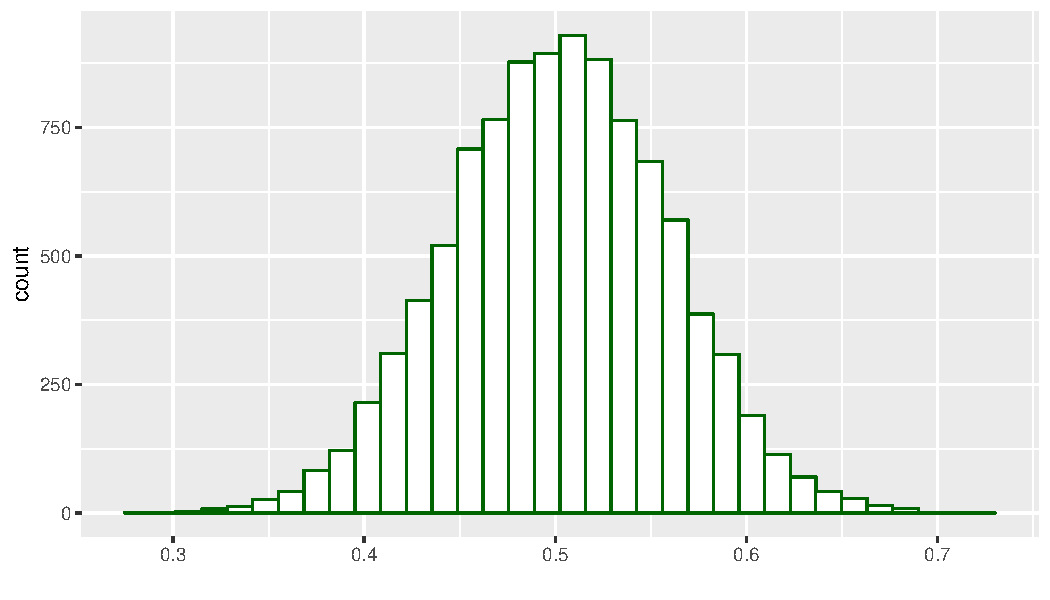
\includegraphics[width=\maxwidth]{figure/unnamed-chunk-1-1} 

\end{knitrout}

  \item Using $\alpha = .05$, what is your decision regarding the viability of the null hypothesis?
  \item Write \emph{one} sentence to President Kroger summarizing what you've learned about the millennials and opinions on same-sex marriage.  
  \ans
\end{enumerate}


% 
% \newpage
% 
% \subsection*{Instructor's Notes}
% 
% <<>>=
% pdata(0.66, vals = ~prop, data = p_hats, lower.tail = FALSE) * 2
% @
% 
% \paragraph{Card Activity}
% 
% \noindent \emph{Learning goals:} gain intuition on establishing and discarding hypotheses based on data, have students generate definition of p-value, insight into why alpha = .05 is used.\\
% 
% \noindent \emph{Materials:} Two decks of cards, a prize of some sort.\\
% 
% Announce that the class is going to play a simple game where every one will have the chance to win the prize. The rules are announced as follows: the instructor will select one student randomly to be the first player.  They'll pick a card from the shuffled deck.  If they pick a red card, they win the prize.  The game keeps going until someone wins the prize.
% 
% Before the class comes in, create a deck of cards that is all black.  Be sure not to show the class while shuffling and fanning the cards for students to choose.  As student after student chooses a black card, you'll start to hear grumbles about how unfair the game is.  They start to get more vocal and articulate after 4 or five cards.
% 
% Once they insist the game stop, you can walk through what happened by writing ``null hypothesis: fair deck; P(red) = 0.5", with the appropriate alternative hypothesis.  In asking why they threw out the null, you'll be able to get them to define a p-value, which you can define formally on the board.  Then you can put up the following probabilities and discuss how .05 is about where they threw out the null.
% 
% <<>>=
% dbinom(0,c(1:5),.5)
% @
% 

\end{document}
